\documentclass[11pt]{book}
\usepackage{caption,graphicx}
\usepackage{float}
\usepackage{indentfirst}
\parskip 5pt    
\usepackage[margin=1in]{geometry}
\setcounter{section}{0}
\renewcommand{\thesection}{\arabic{section}}
\usepackage{amssymb}
\usepackage{enumitem}
\usepackage{setspace}
\usepackage{mathtools}
\linespread{1.0}
\begin{document}
\renewcommand{\labelitemi}{$\textendash$}
\renewcommand{\labelitemii}{{\tiny$\blacksquare$}}
\thispagestyle{plain}

\title{Bachelor's Thesis: Implementing Security in IoT Gateway in Legacy Devices for Telemedicine Applications. A comparison between Lightweight IPsec and CoAP}
\author{Perla Rocío Ramírez Sanabria}
\date{\small{\today}}
\maketitle

\setcounter{tocdepth}{2}
\tableofcontents
\break

\chapter{Introduction}
\chapter{IoT: Internet of Things}
\section{Definition}
The definition of IoT, which stands for Internet of Things, can be expressed as the connection between the ``things" in the physical world and the virtual world, which is the Internet. When the word ``things" is mentioned, it refers to a variety of devices such as mobile phones, wearable devices, RFID among others. In other words, IoT can be understood as an extension of the internet through different devices and systems.\\
It can be defined abstractly by the following statement: ``The IoT refers to the ever-growing network of physical objects that feature an IP address for the internet connectivity and the communication that occurs between these objects and other internet-enabled devices and systems." \\
There are several components necessary for the Internet of Things to exist:
\begin{itemize}
\item \textbf{Sensors:} these are the devices capable of collecting the data processed by the IoT system. They basically detect the different event changes in the environment they are located in. The type of sensor will vary depending on the application, they can measure values such as temperature, moisture, light, acoustic \& noise, movement, water level, presence of chemical substances and among others. After these values are obtained they must be translated into electrical impulses so the system can be able to interpret the data.
\item \textbf{Addressing and identification:} for an IoT system to properly function every operating device requires a unique identifier as well as a unique address, which will make it uniquely identified on the Internet. 
\item\textbf{ Internet Protocol(IP):} it entails a key element because it is the main network protocol used. Currently there exist two versions of this protocol: IPv4 and IPv6. 
\item \textbf{Actuators:} they are the ones in charge of acting according to the data measured by the sensors. These are devices that transform energy into motion and, like sensors, there are different types of motion patterns depending on the kind of energy received such as linear actuators, motors, relays and solenoids.
\item \textbf{IoT gateway:} it is a physical device or software program that serves as a bridge between the data generating devices and the cloud. This component is essential in terms of translating the protocols functioning on the IoT devices into one standard protocol. Regarding the subject on this document, it also improves the security due to a bidirectional management of the data from the cloud to the devices preventing leaks. 
\item \textbf{The cloud:} this is where all the data collected by all the IoT devices are stored and also this is where all the software can access the data for processing.
\item \textbf{User interface:} component required in order to establish a connection between the devices and users. 
\end{itemize}
And different communication channels, which can also be called communication pattern:
\begin{itemize}
\item \textbf{Device-to-Device:} represents the way in which two o more devices connect and communicate directly between each other. Typically this is used with protocols such as Bluetooth, Z-Wave and Zigbee. 
\begin{figure}[H]
	\centering
	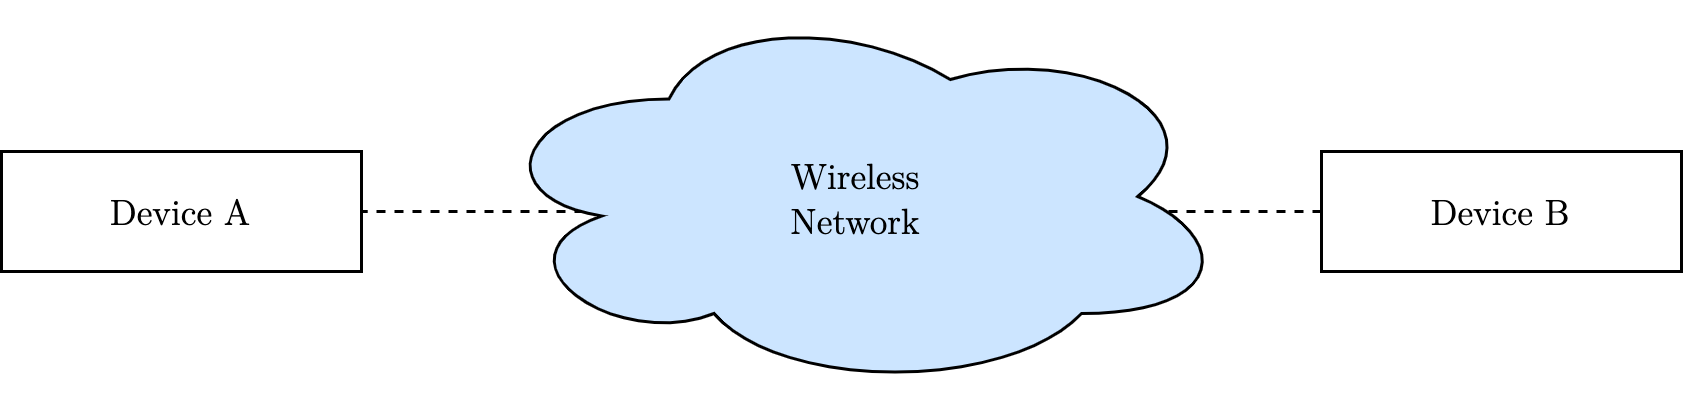
\includegraphics [scale=0.165] {devicedevice.png}
	\caption{Device-to-Device communication pattern representation}
\end{figure}
\item \textbf{Device-to-Cloud:} represents the way in which a device connects directly to the cloud, this can be achieved by wired Ethernet or Wi-Fi connections. 
\begin{figure}[H]
	\centering
	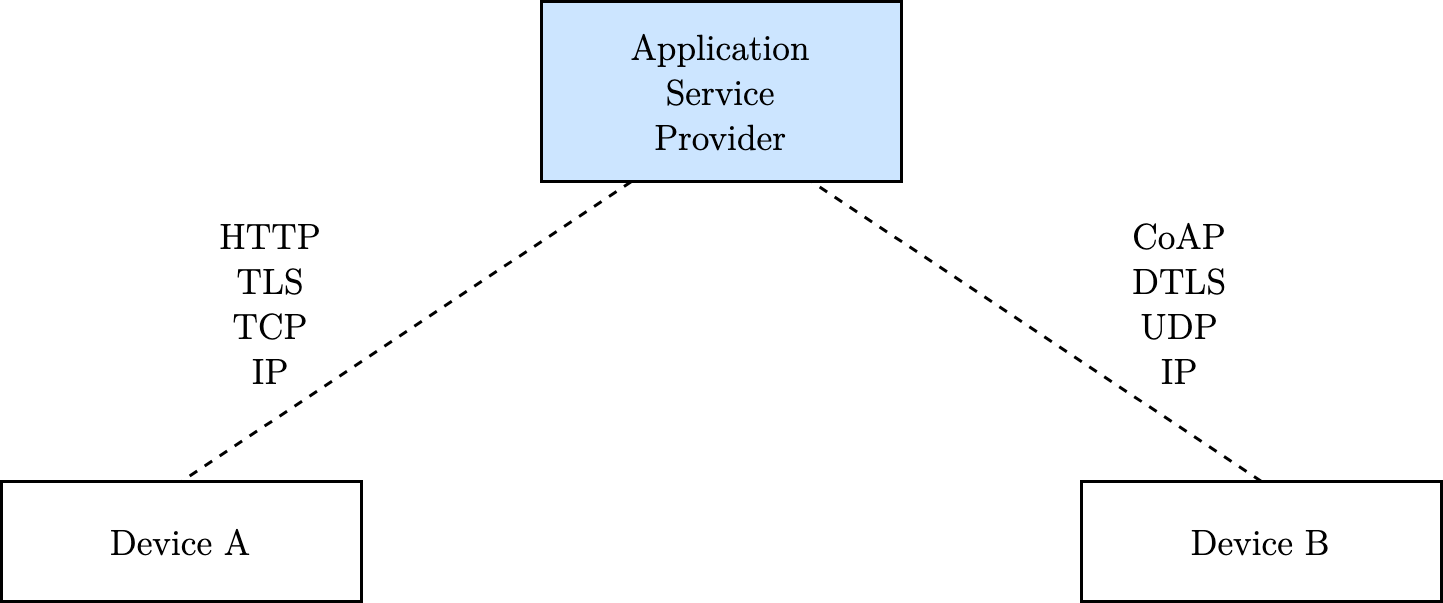
\includegraphics [scale=0.165] {devicecloud.png}
	\caption{Device-to-Cloud communication pattern representation}
\end{figure}
\item \textbf{Device-to-Gateway:} this pattern occurs before the device connects directly to the cloud. It is necessary to translate protocols and add an additional security layer.
\begin{figure}[H]
	\centering
	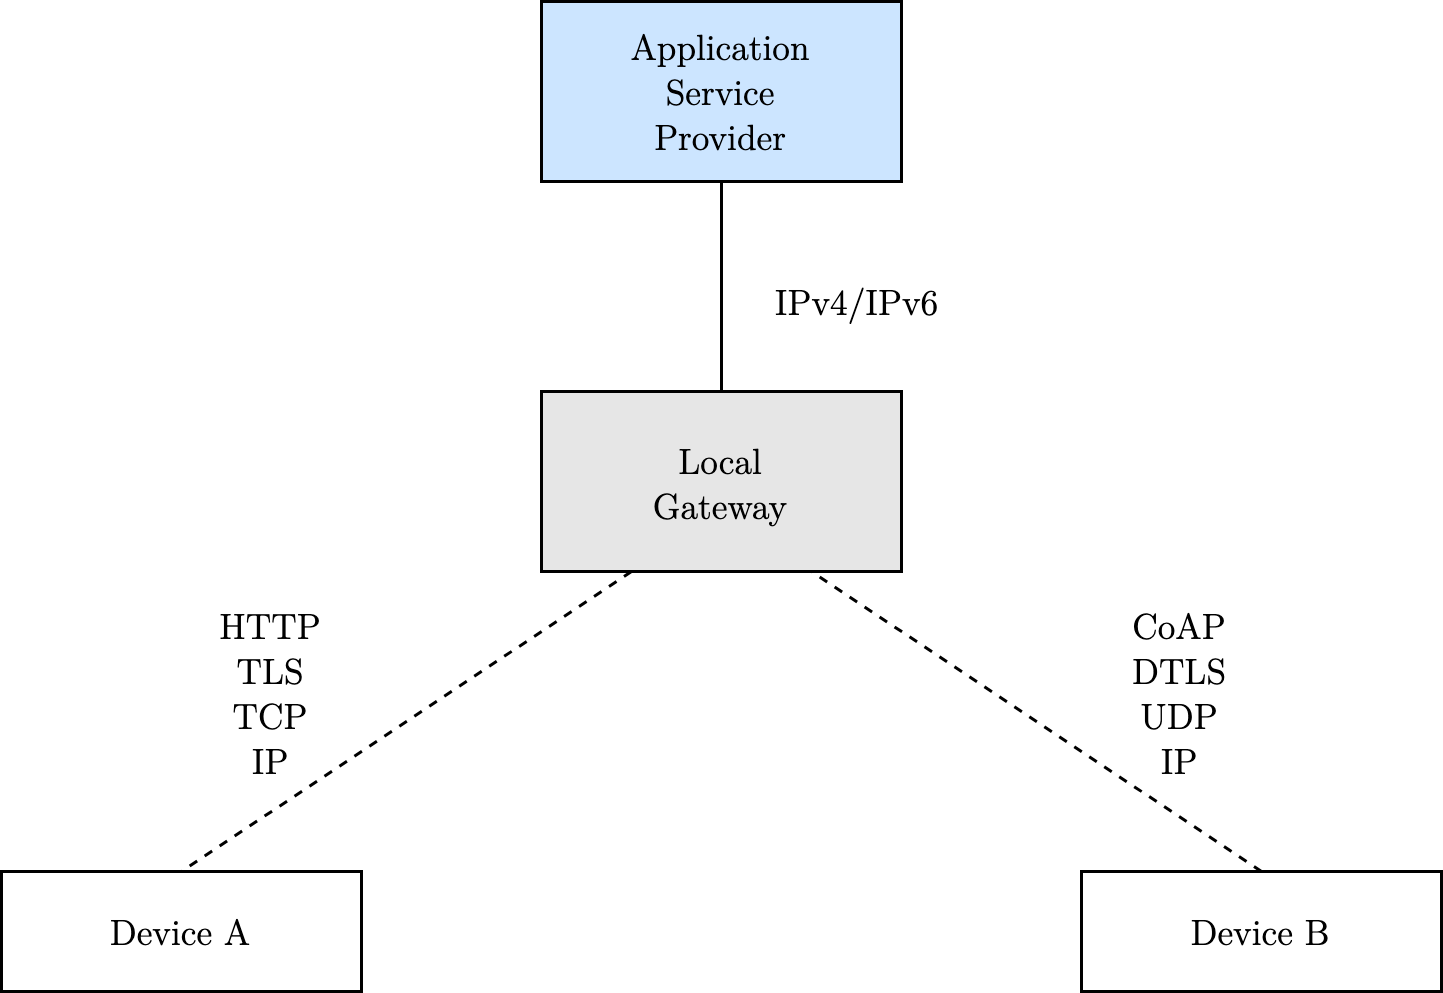
\includegraphics [scale=0.165] {devicegateway.png}
	\caption{Device-to-Gateway communication pattern representation}
\end{figure}
\item \textbf{Back-End Data Sharing:} it works as an extension of the Device-to-Cloud pattern. This enables access for users to later analyse data from different smart devices. 
\begin{figure}[H]
	\centering
	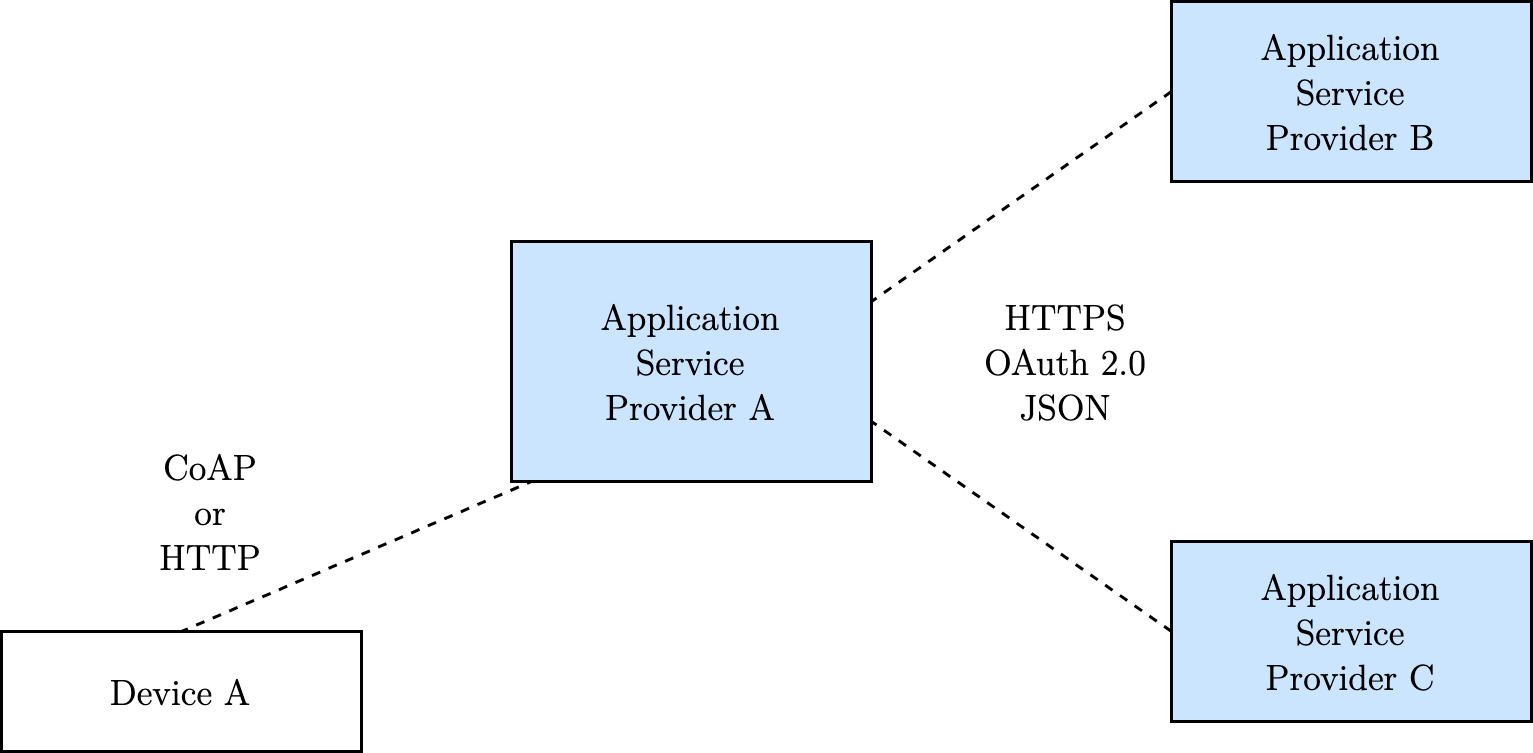
\includegraphics [scale=0.165] {backendsharing.png}
	\caption{Back-End Data Sharing communication pattern representation}
\end{figure}
\end{itemize}

\section{Applications}
IoT covers a wide fan of applications in different sectors thanks to its potential. Nowadays IoT is implemented in a few sectors, but in the future is expected to be implemented in almost every aspect in the citizens life such as personal use, smart homes, cities and hospitals. Some applications are going to be explained briefly below, but the main focus is on the Telemedicine application is going to be explained in detail in the following subsection due to its importance for this thesis. 
\subsubsection{Transportation}
IoT can be extended in terms regarding of the vehicle itself and the driver as well as in different aspects of the transportation system. The different applications in this sector are the following among others:
\begin{itemize}
\item Inter and intra vehicular communications
\item Traffic control.
\item Smart parking.
\item Collision detection.
\item Vehicle control.
\end{itemize}
\subsubsection{Infrastructure Management}
IoT can be utilised in monitoring and control operation of infrastructures such as in bridges and railways. IoT can detect any events or changes that may supposed a risk for the users in said infrastructures. Along with this application, there is also a possibility of using IoT to effectively plan repair and maintenance operations, by organizing duties between different service providers and users of these facilities. Lastly, IoT can be used to control bridges in order to grant access to ships. 
\subsubsection{Home Automation}
This entails what nowadays is called a ``Smart Home". This includes the automation of several devices such as lightning, heating, air conditioning and security systems. Electrical household appliance are also included here such as fridges, washing machines, dryers or ovens. 
\subsubsection{Media, Entertainment.}
It is known as Multimedia-IoT and it refers to the different technologies used in order to transmit media information. This can go from certain streaming services to surveillance material. 
\subsection{Application: Telemedicine/Medical and Health Care}
\chapter{IPsec: Internet Protocol Security}
\section{Definition}
IPsec results from the abbreviation of Internet Protocol Security. This protocol provides a framework of open standards to ensure secure communications over IPv4 or IPv6, authenticating and encrypting each packet, thus ensuring communications at the network level and at all higher levels. Being optional for IPv4 and mandatory for IPv6.\\
IPsec can be implemented in several ways such as:
\begin{itemize}
\item Site-to-Site Connections (Networks Interconnection)
\item Host-to-Host Connections
\item Host-to-Site Connections (Remote Access)
\end{itemize}
And there exist several benefits about implementing IPsec:
\begin{itemize}
\item Transparent for protocols such as TPC and UPD as well for users and applications.
\item It improves the security provided by other mechanisms such as SSL, TLS or SSH, operating all these at level 4 or higher.
\item Possibility of integrating it into a perimeter security device.
\end{itemize}


\section{Modes}
IPsec operates in two possible modes, transport or tunnel which are going to be discussed in the following subsections.
\subsection{Transport}
When working with this mode the original IP packet is modified by inserting an additional header between the network and transport layer only protecting the information coming from the transport layer. 
\begin{figure}[H]
	\centering
	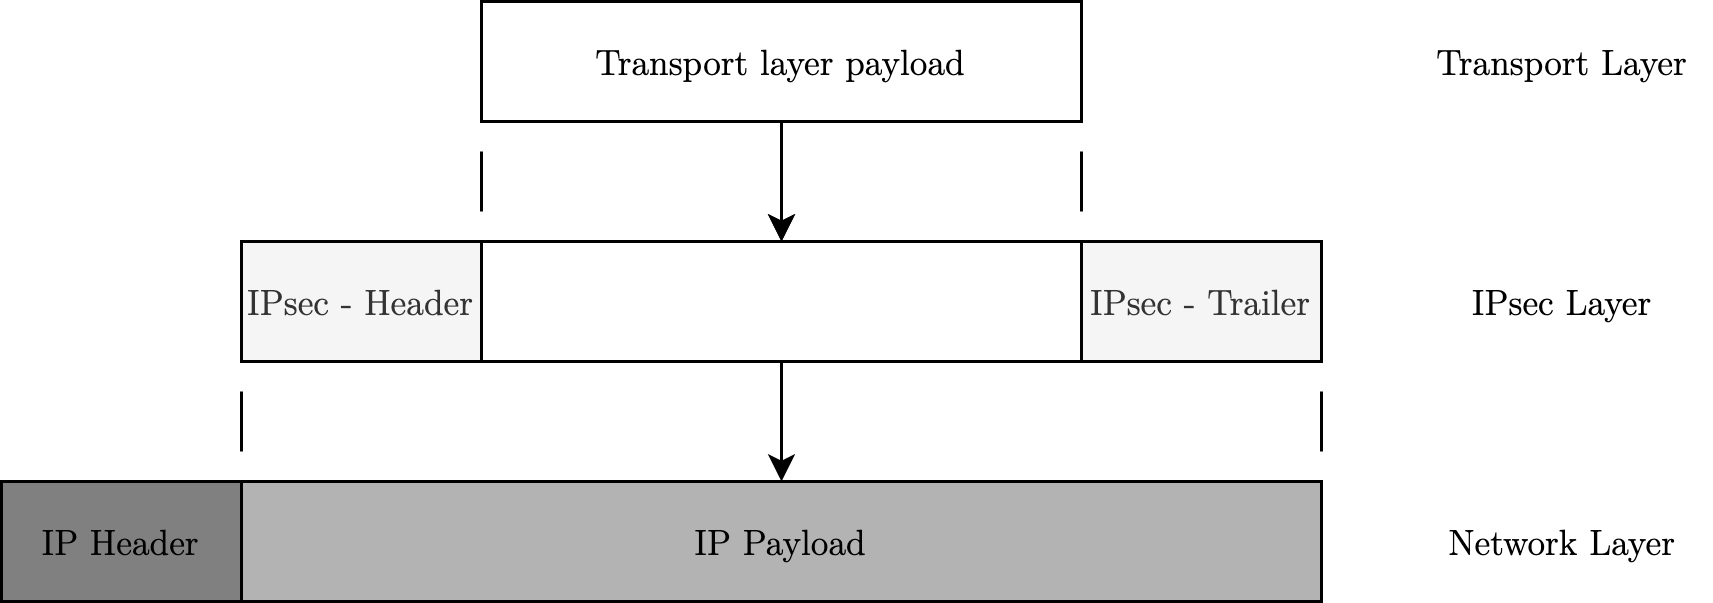
\includegraphics [scale=0.165] {transport_encapsulation.png}
	\caption{IPsec in transport mode}
\end{figure}
As it can be seen, the segment of the transport layer is encapsulated with a header and a trailer, this resulting encapsulation will be the final IP packet data field where the source and destination IP addresses are those of the two nodes that want to communicate securely.\\

\subsection{Tunnel}
When working with this mode the original IP packet is encapsulated entirely in a new IP packer, where the new IP header will have as origin and destination addresses the ends of the tunnel. Therefore, the entire packet is protected unlike when working with the transport mode. 
\begin{figure}[H]
	\centering
	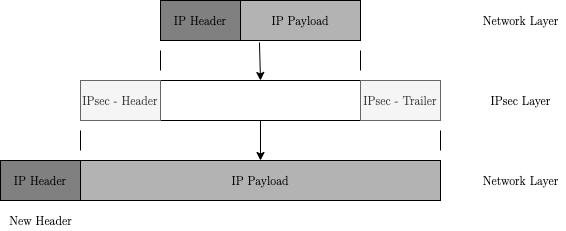
\includegraphics [scale=0.165] {tunnel_encapsulation.png}
	\caption{IPsec in tunnel mode}
\end{figure}
In tunnel mode it is the original IP packet the one being encapsulated with an IPsec header and a trailer. A new IP header is added to the resulting encapsulation, where, as already said before, the source and destination IP addresses are those at the ends of the tunnel.
\section{Components of IPsec}
\subsection{Security Protocols}
\subsubsection{AH: Authentication Header}
The AH security protocol provides authentication and integrity to the IP packets transmitted, but without encryption. This means that there is a guarantee that the data was sent by a legitimate sender and it has not been altered, but there is no guarantee for confidentiality. This will also prevent IP packets' replay and at the same time it protects immutable fields in IP header.\\
In order to protect the IP header and data against modifications, a MAC (Message Authentication Code) function is applied to the majority of the bytes of the IP datagram, except for the fields that could change such as TOS, Flags, Checksum and TTL fragments offset. The minimum requirements for this MAC function are HMAC-MD5-96 and HMAC-SHA-1-96.
\begin{figure}[H]
	\centering
	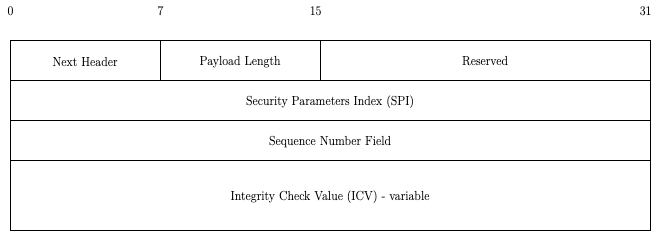
\includegraphics [scale=0.175] {ah_fields.png}
	\caption{AH fields}
\end{figure}

The AH extension contains the following fields:
\begin{itemize}
\item \textbf{Next Header:} this field is 1 byte long and it is used in order to identify the type of the next payload after the Authentication Header. The value assigned to this field will vary depending on the protocol used and it is chosen from the set of IP Protocol Number that is defined by the IANA. For example, 1 for ICMP, 6 for TCP, 17 for UDP, etc. 
\item \textbf{Payload Length:} this field is 1 byte long and it is used to specify the length of AH in multiples of 4 bytes (32 bits), excluding the first 8 bits.
\item \textbf{Reserved:} this field is 2 bytes long and it is reserver for future use. Since it is not used currently, the sender must set a value ``0" for this field and it should be ignored by the recipient. 
\item \textbf{Security Parameters Index (SPI):} this field is 4 bytes long and it is used to identify the SA (Security Association), which will be discussed later in this document. 
\item \textbf{Sequence Number:} this field is 4 bytes long and it contains a counter value for all the packets sent, this means that with every packet sent this value will increase. The sender must include even if the recipient does not activate the anti replay protection, in which case it will be ignored by the latter.
\item \textbf{Extended Sequence Number (ESN):} this field is 8 bytes long and it is used to support high-speed IPsec implementations by at the same time prolonging a SA's lifetime. This ESN must be negotiated when SA is created by the SA management protocol. This works as an extension of the already existing 4 bytes sequence number field.
\item \textbf{Integrity Check Value (ICV):} this field has a variable length and it contains the ICV, which will provide authentication and integrity checking. Its length must be an integral multiple of 32 bits for both IPv4 and IPv6. 
\end{itemize}

\break

In the following figures we can see the AH encapsulation with the two possible modes:
\begin{figure}[H]
	\centering
	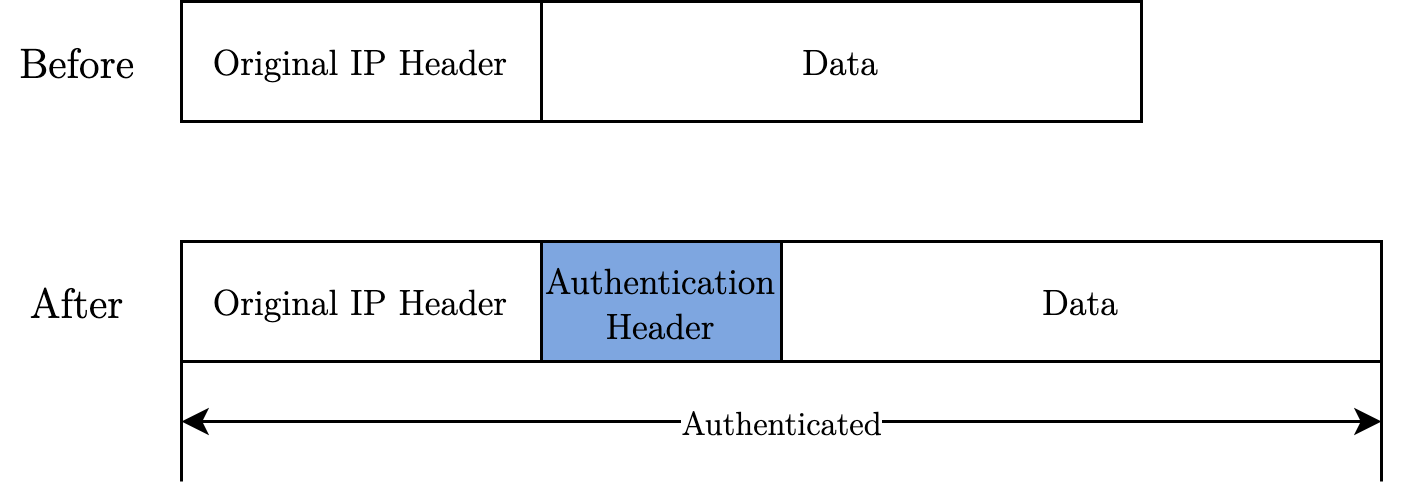
\includegraphics [scale=0.17] {ah-transport.png}
	\caption{AH Encapsulation in transport mode}
\end{figure}
\begin{figure}[H]
	\centering
	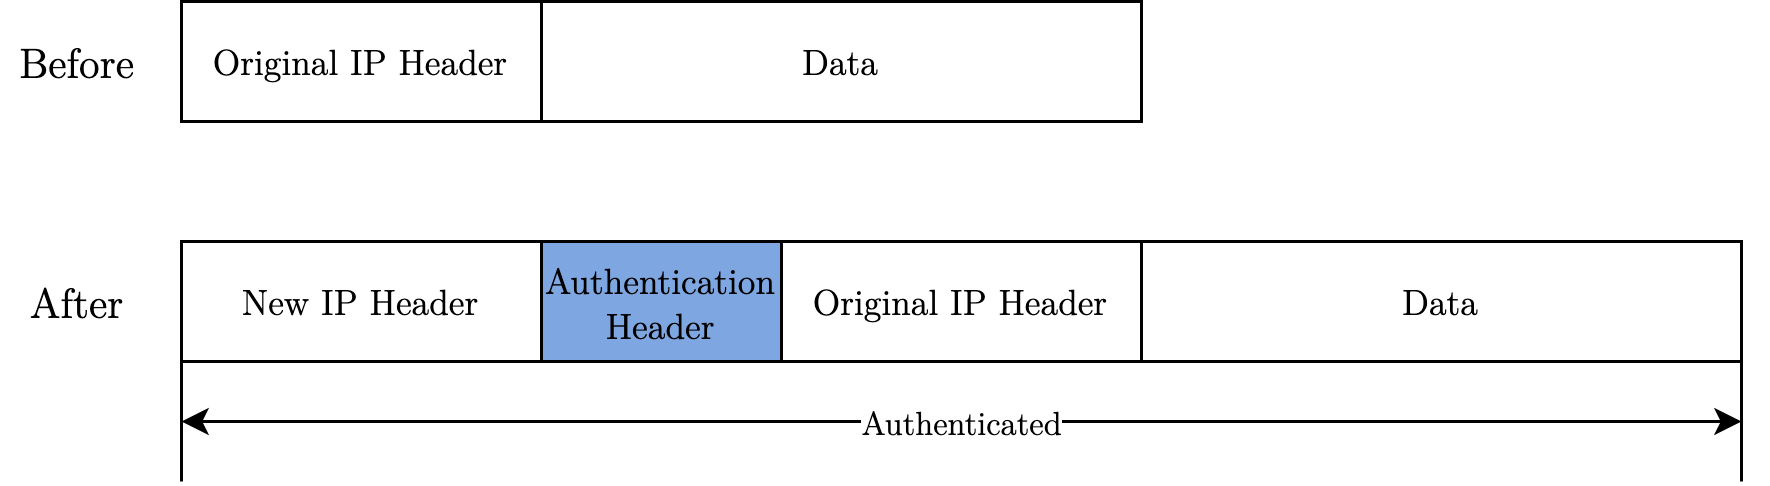
\includegraphics [scale=0.17] {ah-tunnel.png}
	\caption{AH Encapsulation in tunnel mode}
\end{figure}

\subsubsection{ESP: Encapsulating Security Payload}
The ESP security protocol provides data integrity, source authentication and confidentiality of IP packets. However, ESP does not provide integrity and authentication for the entire IP packet, which is the reason why there exist the possibility to combine it with AH.\\
It guarantees that the content cannot be examined by third parties or, if possible, that it cannot be interpreted. It will be necessary to use a key in order to encrypt the data and different encryption algorithms can be used, such as DES, 3DES, RC5, etc. \\
It is important to note that ESP does not encrypt nor authenticate the IP header fields unless they are encapsulated by ESP using the tunnel mode. 
\begin{figure}[H]
	\centering
	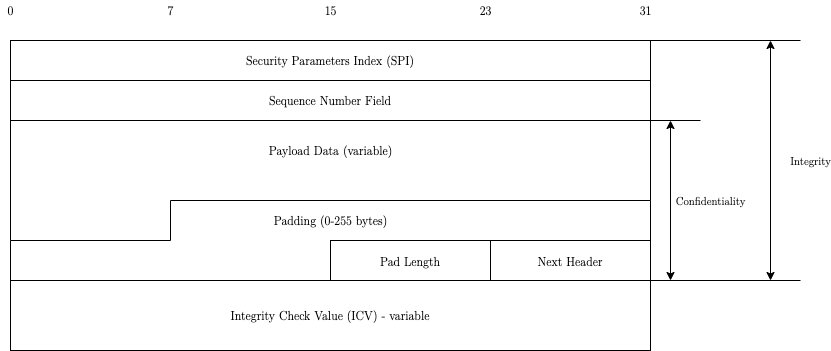
\includegraphics [scale=0.165] {esp_header.png}
	\caption{ESP fields}
\end{figure}
The ESP extension contains the following fields:
\begin{itemize}
\item \textbf{ESP Header:} 
	\begin{itemize}
	\item \textbf{Security Parameters Index (SPI):} this field is 4 bytes long and it is used to identify the SA (Security Association), which will be discussed later in this document. 
	\item \textbf{Sequence Number:} this field is 4 bytes long and it contains a counter value for all the packets sent, this means that with every packet sent this value will increase. The sender must include even if the recipient does not activate the anti replay protection, in which case it will be ignored by the latter.
	\item \textbf{Extended Sequence Number (ESN):} this field is 8 bytes long and it is used to support high-speed IPsec implementations by at the same time prolonging a SA's lifetime. This ESN must be negotiated when SA is created by the SA management protocol. This works as an extension of the already existing 4 bytes sequence number field.
\end{itemize}
\item \textbf{Payload Data:} this field has a variable length that will vary depending on the length of the data. Contains data described by the Next Header field as well as the initialisation vector for the encryption algorithm. It is the information that is actually protected by ESP.
\item \textbf{ESP Trailer:}
	\begin{itemize}
	\item \textbf{Padding:} there are two factors why this field is needed: 
		\begin{enumerate}
		\item The requirement for the plaintext to be a multiple of a certain number.
		\item The requirement for the resulting ciphertext to terminate on a 4-byte boundary.
		\end{enumerate}
	This field has a variable length that can go from 0 to 255 bytes depending on the requirements needed. 
	\item \textbf{Pad Length:} this field is 1 byte long and it is used to specify the length of the previously mentioned padding. It accepts values from 0 to 255, where a ``0" value indicates the absence of Padding bytes.
	\item \textbf{Next Header:} this field is 1 byte long and it is used in order to identify the type of the next payload after the Authentication Header. The value assigned to this field will vary depending on the protocol used and it is chosen from the set of IP Protocol Number that is defined by the IANA. For example, 1 for ICMP, 6 for TCP, 17 for UDP, etc. 
	\end{itemize}
\item \textbf{Integrity Check Value:} this field has a variable length and it is the result of the computation over the ESP header, Payload, and ESP trailer fields.
\end{itemize}
In the following figures we can see the ESP encapsulation with the two possible modes:
\begin{figure}[H]
	\centering
	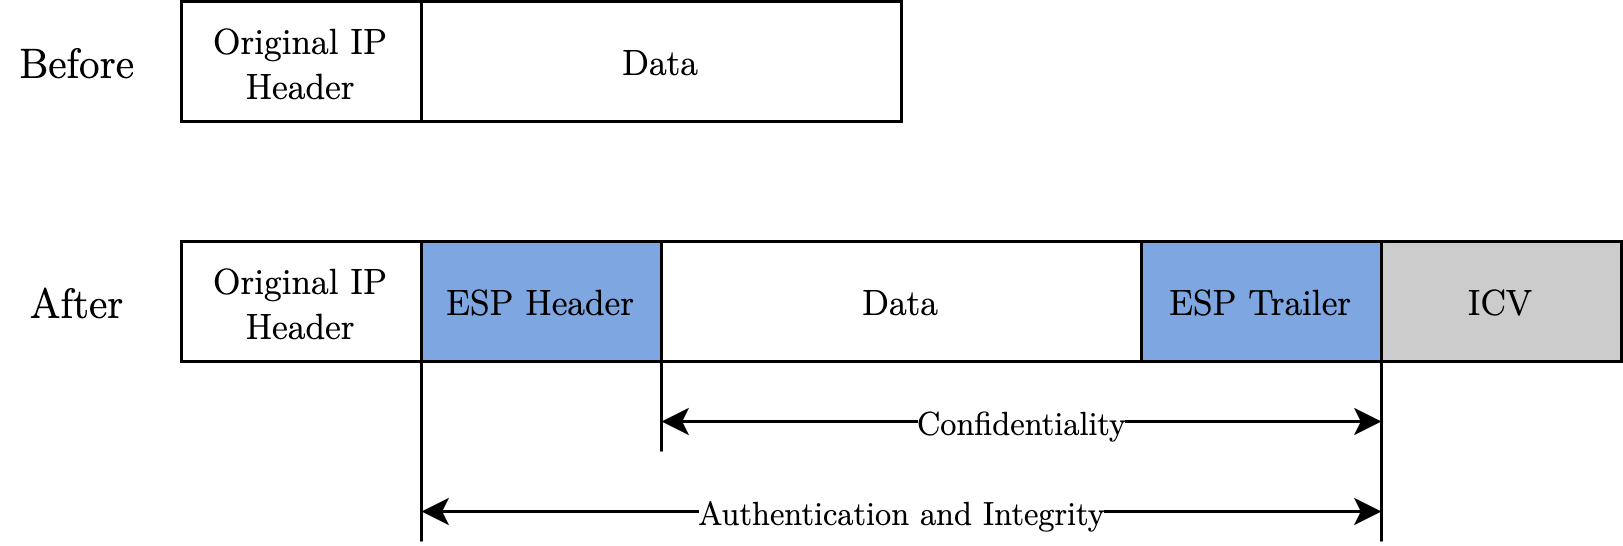
\includegraphics [scale=0.175] {esp-transport.png}
	\caption{ESP Encapsulation in transport mode}
\end{figure}
\begin{figure}[H]
	\centering
	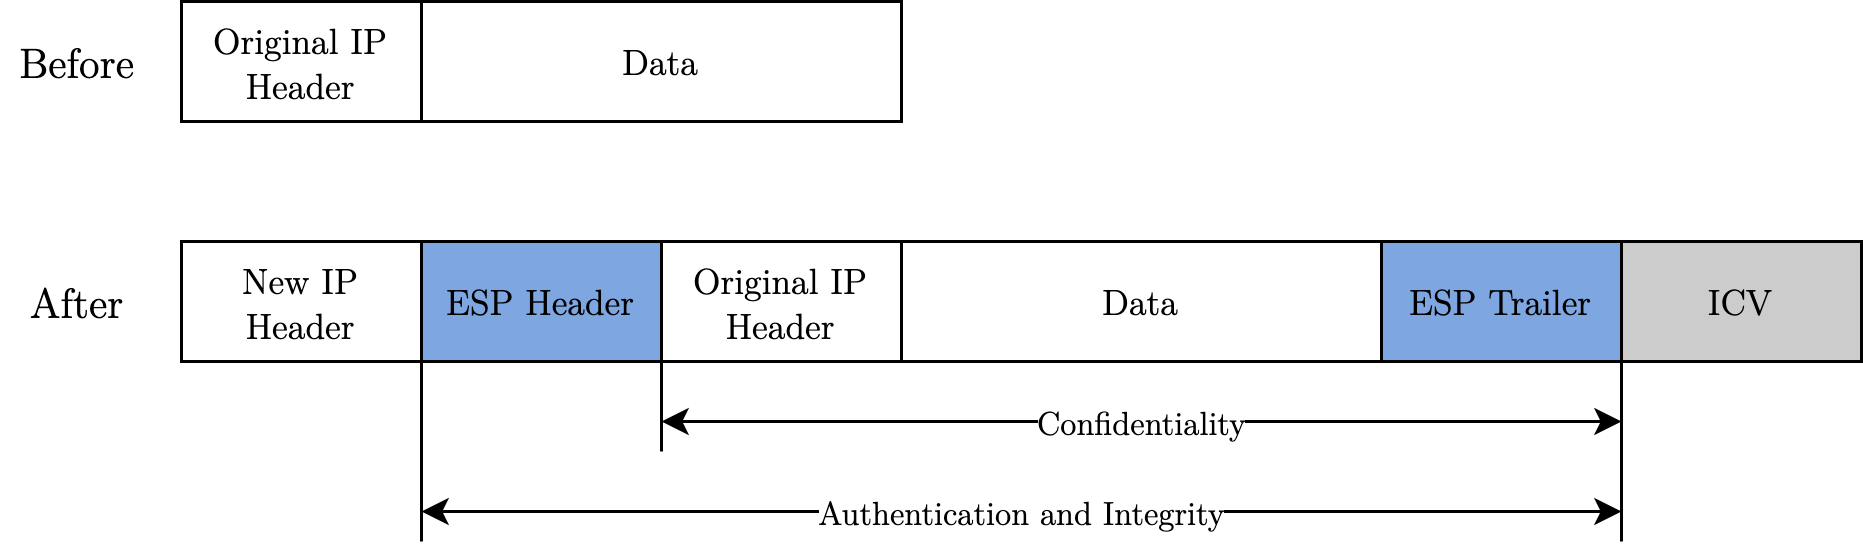
\includegraphics [scale=0.175] {esp-tunnel.png}
	\caption{ESP Encapsulation in tunnel mode}
\end{figure}


\subsubsection{ Security Associations}
An IPsec Security Association specifies the security properties for the traffic between the parties in a communication. Within these SAs the needed parameters such as encryption algorithms or keys are negotiated. These SAs are created dynamically by the Internet Key Exchange (IKE) protocol, which is going to be discussed in more detail later in the document.\\
An SA constitutes a simplex connection, which means that if the connection needs to be protected in both ways two SA's are required. Additionally, in every SA there is a possibility to use AH and ESP, but not simultaneously. Therefore, two SAs are required for each direction if both security protocols are used.\\
There are three parameters that defines an SA uniquely:
\begin{itemize}
\item Security Parameter Index (SPI)
\item Destination IP Address (DA)
\item Protocol identifier (P)
\end{itemize}
The three values previously mentioned are included in the data sent and in the Security Association Database (SAD) as we can see in the figure below:
\begin{figure}[H]
	\centering
	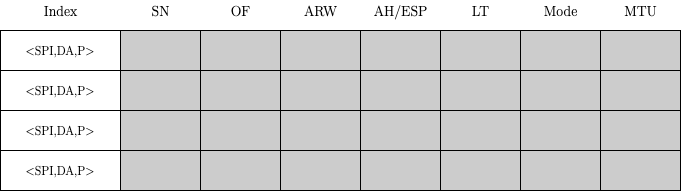
\includegraphics [scale=0.165] {sadb_table.png}
	\caption{Security Association Database}
\end{figure}
A Security Association Database (SAD) a central repository that contains all the active SAs for both inbound and outbound processes. With each entry on the database the specific parameters for each SA are defined.
\begin{itemize}
\item \textbf{SN (Sequence Number):} 32-bit value used to generate sequence numbers for the security protocols.
\item \textbf{OF (Overflow Flag)}
\item\textbf{ ARW (Anti-Replay Window):} detects inbound replayed packet.
\item \textbf{AH/ESP:} 
	\begin{itemize}
	\item AH Information: Authentication algorithm, Keys, Key lifetime, others.
	\item ESP Information:Encryption algorithm, Authentication algorithm, Keys, Key lifetime, Initialisation vectors, others.
	\end{itemize}

\item \textbf{LT (Lifetime):} specifies the lifetime for the SA.
\item \textbf{Mode:} specifies the mode, which can be transport or tunnel.
\item \textbf{MUT(Path MTU):} specifies the path MTU. 
\end{itemize}


\section{Key Management. Internet Key Exchange (IKE)}
The IKE protocol is not a part of the IPsec specification, but it is integrated with it. As it was stated before in this document, it is the one in charge to create SAs, negotiate security policies, perform key exchange and authenticate the nodes.\\
It is a hybrid protocol based on the framework defined by Internet Security Association and Key Management Protocol (ISAKMP) and two other key management protocols: Oakley and SKEME. The latter protocols define a method with a view to establish an authenticated key exchange. The tasks for these protocols are:
\begin{itemize}
\item \textbf{ISAKMP:} provides a framework for authentication and key exchange by defining the format of the messages.
\item \textbf{Oakley:} It is the protocol for determining symmetric keys, based on Diffie-Hellman, but with additional security.
\item \textbf{SKEME:} ``describes a versatile key exchange technique which provides anonymity, repudiability, and quick key refreshment" (RFC IKE)
\end{itemize}
Regarding the authentication, there two possible techniques:
\begin{itemize}
\item \textbf{Pre-Shared Key (PSK)}, from which an authentication hash is created and exchanged between the parties.
\item \textbf{RSA Signature}, a hash is signed with the private key and then exchanged  between the parties. 
\end{itemize}
It divides its activity into two phases:
\begin{itemize}
\item \textbf{PHASE 1:} Negotiation of the IKE SA to protect phase 2 and it has two possible modes: main and aggresive.
\item \textbf{PHASE 2:} Negotiation of SA for a data exchange protocol, in our case IPsec in each flow.
\end{itemize}

\break

In the following figures we can se the two phases implementing both modes for PHASE 1:
\begin{figure}[H]
	\centering
	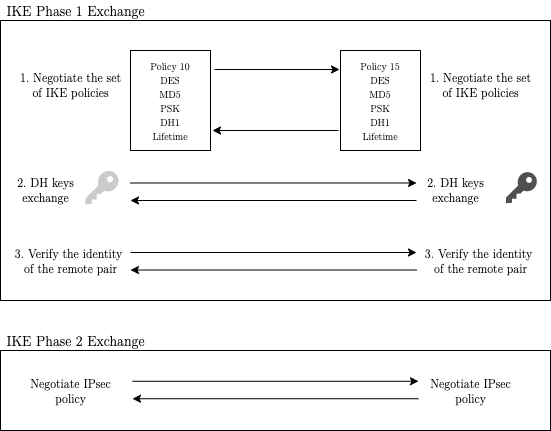
\includegraphics [scale=0.19] {main.png}
	\caption{IKE: Phase 1 and Phase 2}
\end{figure}

\begin{figure}[H]
	\centering
	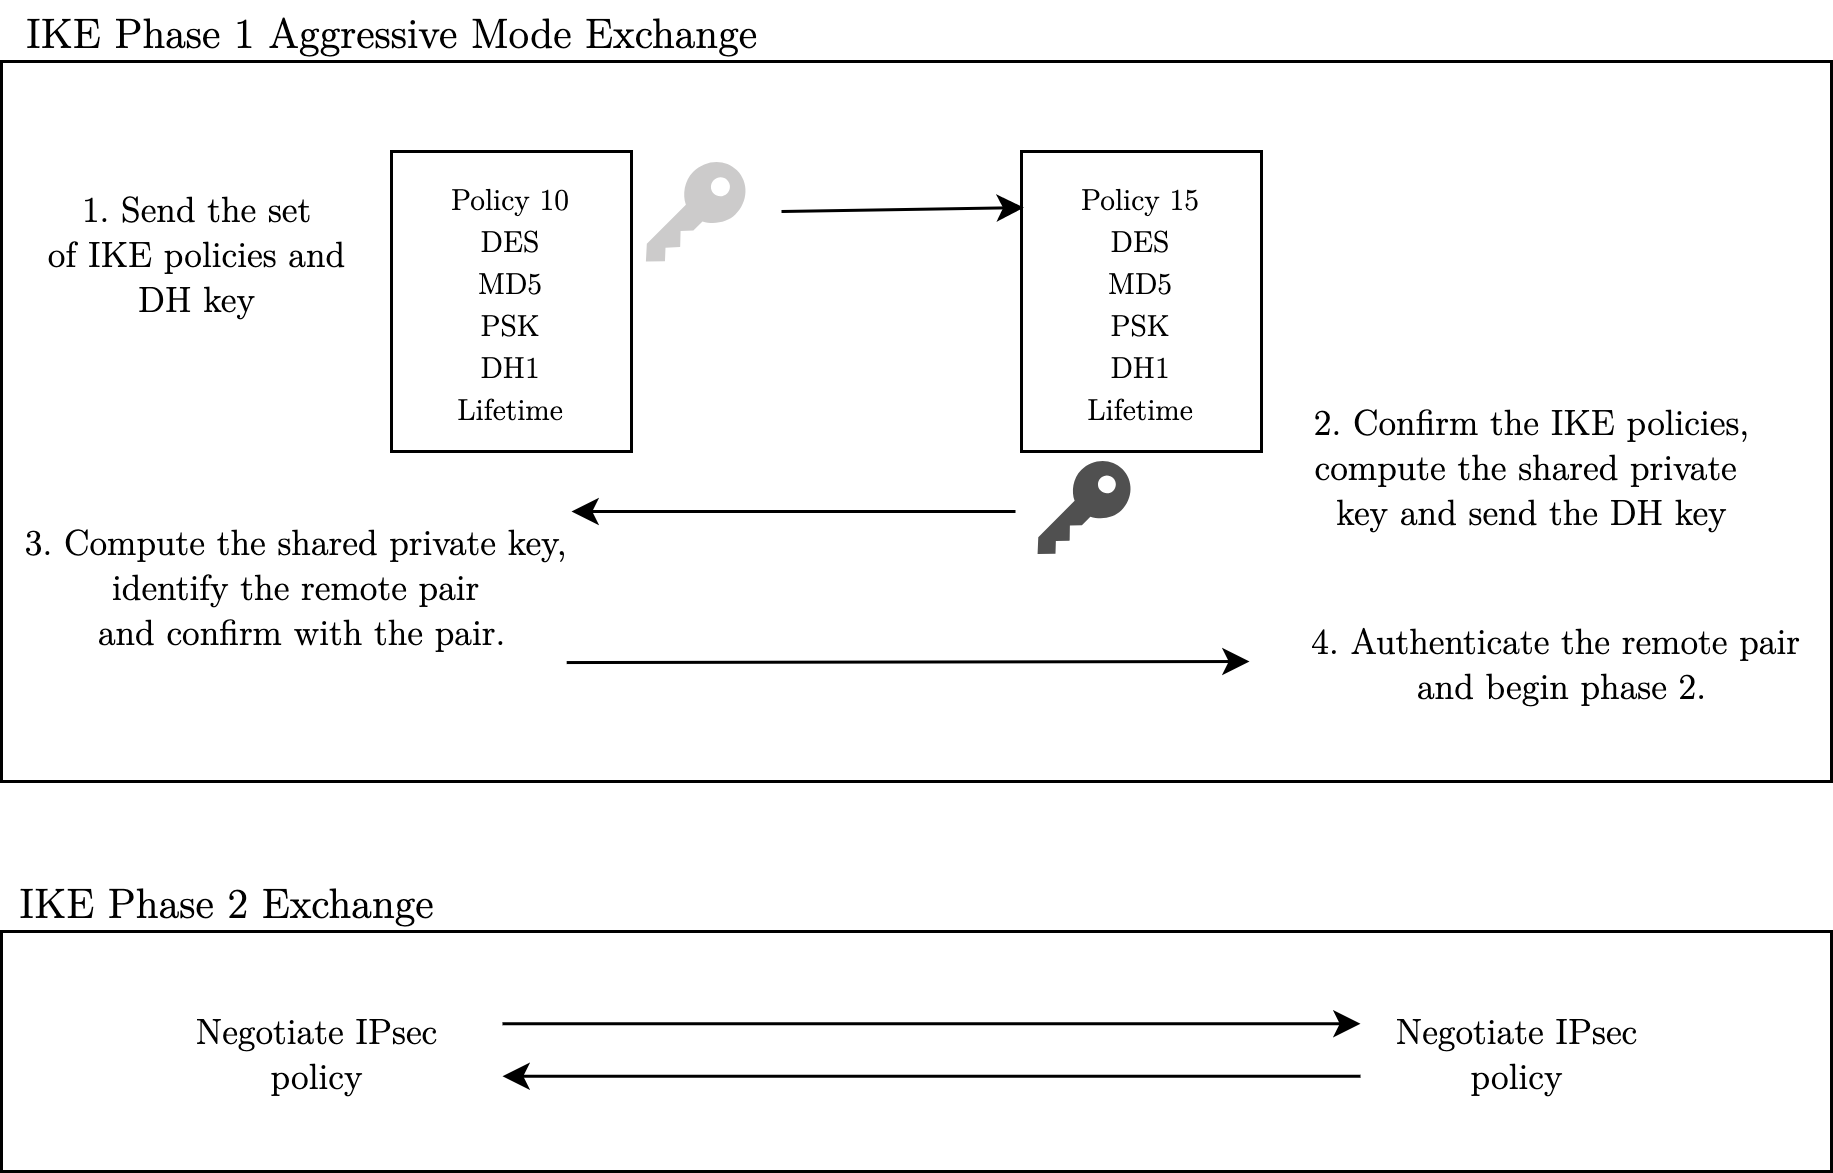
\includegraphics [scale=0.19] {aggressive.png}
	\caption{IKE: Phase 1 (Aggressive Mode) and Phase 2}
\end{figure}

\break

Finally in the following figure we can see the different algorithms used in order to establish a secure communication between two (or more) parties via IPsec implementation:

\begin{figure}[H]
	\centering
	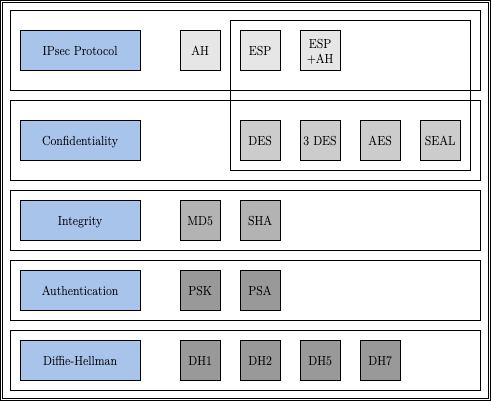
\includegraphics [scale=0.175] {summary.png}
	\caption{Algorithms}
\end{figure}
\section{Lightweight IPsec}
\chapter{CoAP: Constrained Application Protocol}
\section{Definition}
According to the document RFC 7252 where this protocol is defined: ``The Constrained Application Protocol (CoAP) is a specialised web transfer protocol for use with constrained nodes and constrained (e.g., low-power, lossy) networks." The main function of this protocol is to enable easy, limited devices to access the IoT in constrained networks which usually present low availability and bandwidth. \\
CoAP is an application layer protocol designed similarly to the Hypertext Transfer Protocol (HTTP), this ensures compatibility in terms of the REST model with the latter protocol even using the same methods (GET, POST, PUT and DELETE), URIs, MIME types, etc. The main reason behind this is for an easy translation between both CoAP and HTTP as well as to a simple integration in the web. The main differences with HTTP are located within the security framework. \\
\begin{figure}[H]
	\centering
	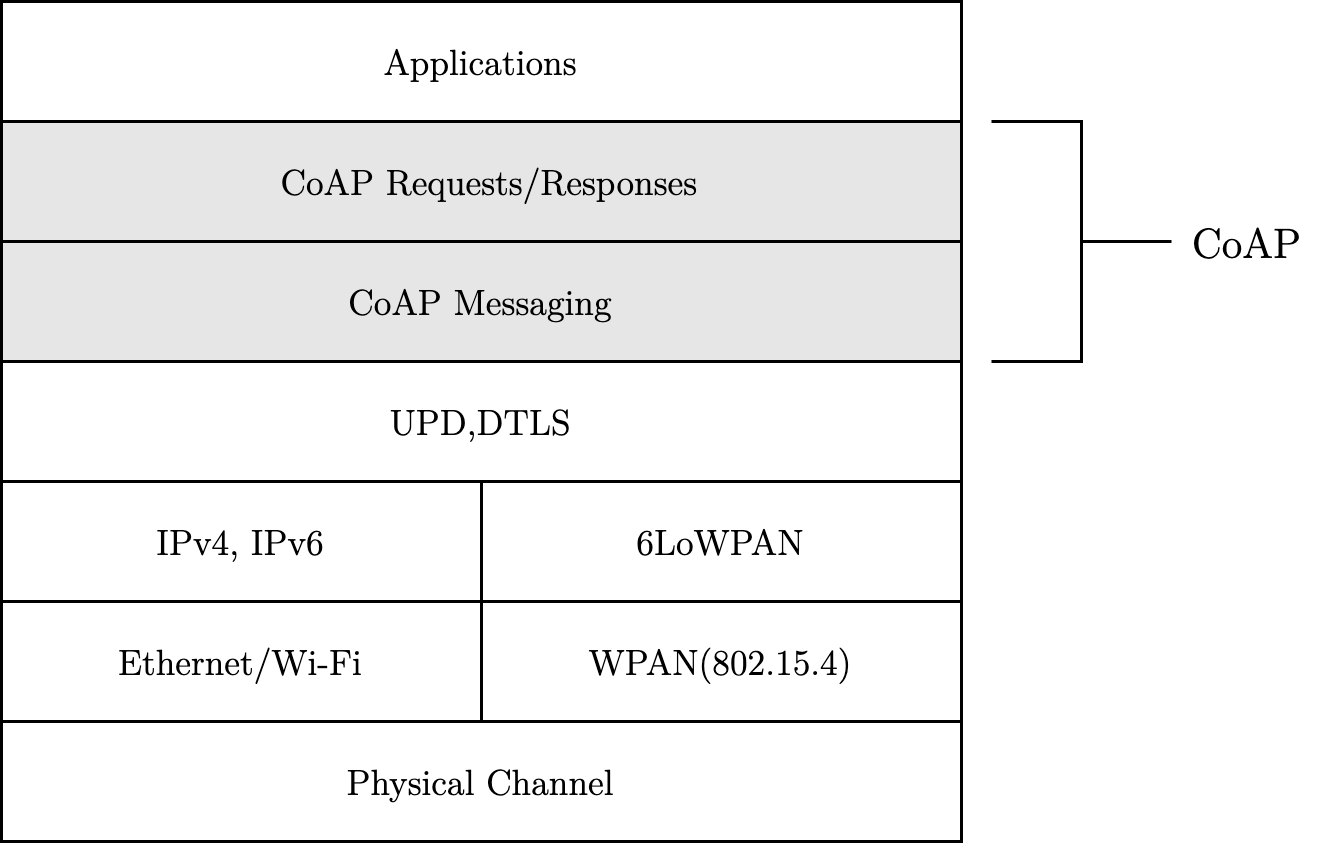
\includegraphics [scale=0.175] {coapstack.png}
	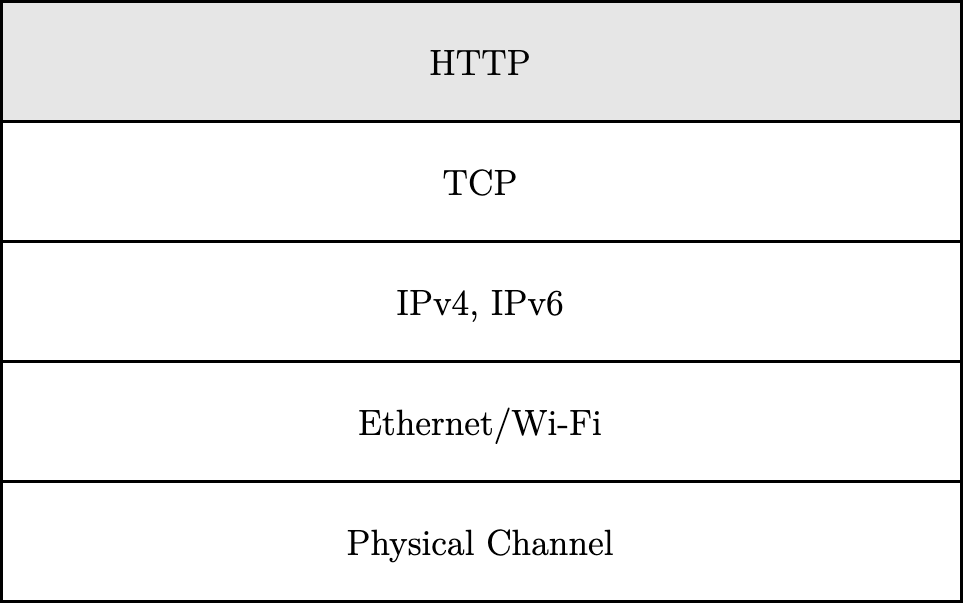
\includegraphics [scale=0.175] {httpstack.png}
	\caption{Comparison between Secured-DTLS CoAP Stack and HTTP Stack}
\end{figure}
CoAP presents a series of features, which are the following:
\begin{itemize}
\item Constrained web protocol fulfilling M2M requirements.
\item Security binding to DTLS (Datagram Transport Layer Security).
\item Asynchronous message exchanges.
\item Low header overhead and parsing complexity.
\item URI and Content-Type support. 
\item Simple proxy and caching capabilities.
\item A stateless HTTP mapping, allowing proxies to be built providing access to CoAP resources via HTTP in a uniform way or for HTTP simple interfaces to be realised alternatively over CoAP.
\end{itemize}
\section{CoAP Structure Model}
\subsection{Messaging Model}
The CoAP message exchange is carried out on UPD endpoints and there are four possible messages which are: \begin{itemize}
\item CON (Confirmable)
\item NON (Non-confirmable)
\item ACK (Acknowledgemente)
\item RST (Reset)
As well as different types of transport:
\begin{itemize}
\item \textbf{Reliable message transport}\\
Message transport acquires reliability by marking the message sent by the client as Confirmable. The client sends the messages periodically until it receives an Acknowledgement message (ACK) message with the same Message ID from the server. 
\begin{figure}[H]
	\centering
	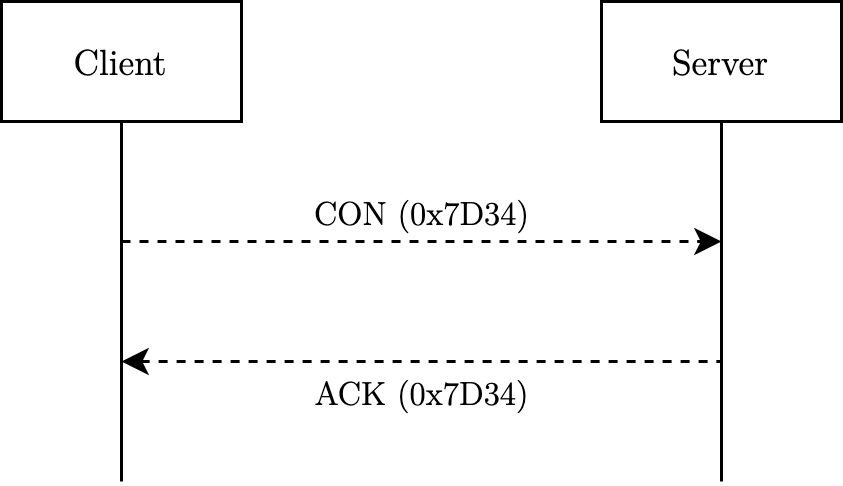
\includegraphics [scale=0.175] {messagingmodel.png}
	\caption{Reliable Message Transmission}
\end{figure}
If the recipient is not able to process a Confirmable (CON) message, it replies with a Reset message (RST) instead of an Acknowledgement message (ACK).
\item \textbf{Unreliable message transport}\\
There is also a possibility to obtain an unreliable transmission by marking the message sent by the client as Non-confirmable. In this case, the client does not wait for an Acknowledgement message (ACK) from the server. However, Message ID is included for detection in case duplication occurs. 
\begin{figure}[H]
	\centering
	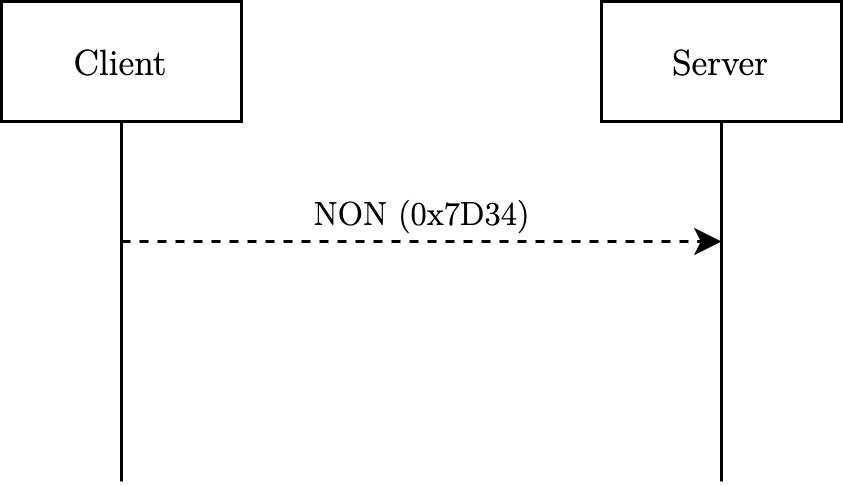
\includegraphics [scale=0.175] {unmessaging.png}
	\caption{Reliable Message Transmission}
\end{figure}
If the recipient is not able to process a Non-confirmable message, it may reply with a Reset message (RST).
\end{itemize}
\end{itemize}
\subsection{Message Format}
\begin{figure}[H]
	\centering
	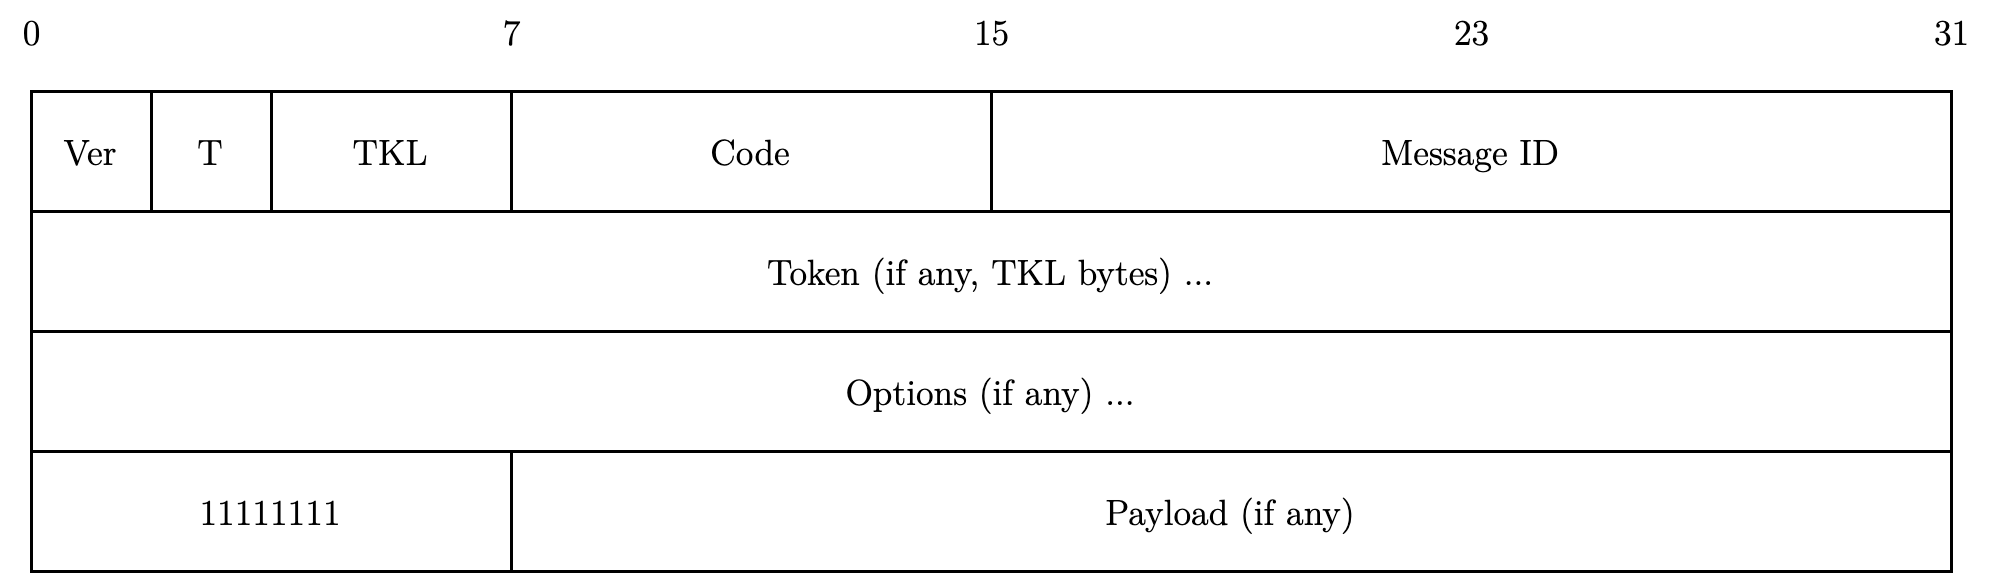
\includegraphics [scale=0.175] {messageformat.png}
	\caption{Message Format}
\end{figure}
The fields in a CoAP message are:
\begin{itemize}
\item \textbf{Version (Ver):} this field, coded on 2 bits (unsigned), indicates the CoAP version. Implementations of this specification MUST set this field to 1 (01 binary).  Other values are reserved for future versions. 
\item \textbf{Type (T):} this field, coded on 2 bits (unsigned), indicates the message type Confirmable (0), Non-confirmable (1), Acknowledgement (2), or Reset (3).
\item \textbf{Token Length (TKL):} this field, coded on 4 bits (unsigned), indicates the length of the variable-length Token field (0-8 bytes). 
\item \textbf{Code:} this field coded on 8 bits (unsigned) is split in two parts as its syntax is c.dd:
	\begin{itemize}
	\item \textbf{c:} Class. 3 bits. Digit from 0 to 7
	\item \textbf{dd:} Details. 5 bits. Digit from 0 to 31
	\end{itemize}
The class can indicate a request (0), a success response (2), a client error response (4), or a server error response (5)
\item \textbf{Message ID:} this field, coded on 16-bit unsigned integer in network byte order, is used to detect message duplication and to match messages of type Acknowledgement/Reset to messages of type Confirmable/Non-confirmable.
\item \textbf{Token:}  this field, which may be 0 to 8 bytes, is used to correlate requests and responses.
\item \textbf{Options:} Both requests and responses may include a list of one or more options. These are some possible options: Content-Format, ETag, Location-Path, Proxy-Uri, If-Match, Uri-Query.
\end{itemize}
\subsection{Request/Response Model}
In the CoAP messages exchanged a Method Code or Response Code are going to be included mandatorily in a request and response respectively. Optionally, information such as URI and payload media type are carried as options. \\
A request can be carried out with a Confirmable (CON) or Non-confirmable (NON) message. When the message used by the client is Confirmable (CON) there exist two ways of obtaining a response:
\begin{itemize}
\item \textbf{Piggybacked:} when the response is received immediately.
\begin{figure}[H]
	\centering
	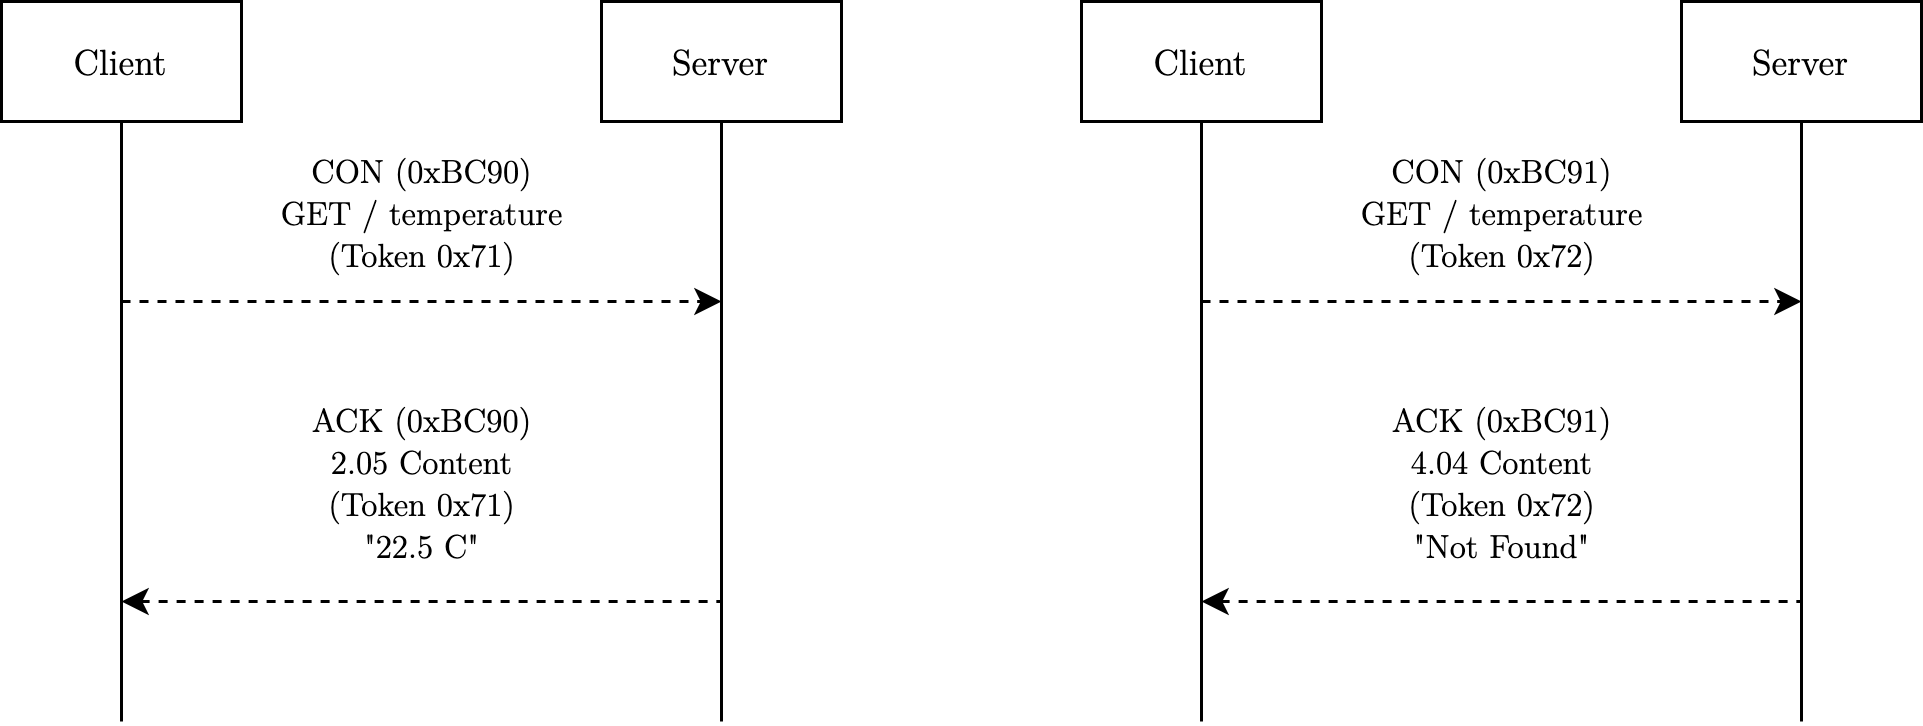
\includegraphics [scale=0.175] {request-response.png}
	\caption{Two GET Requests with Piggybacked Responses. Success and Failure.}
\end{figure}
\item \textbf{Separate Response:} this occurs when the server is not able to respond immediately, the first response is going to be an empty Acknowledgement message (ACK) so the client does not retransmit the request again. Once the response is ready, the server sends the information as a Confirmable (CON) message.
\begin{figure}[H]
	\centering
	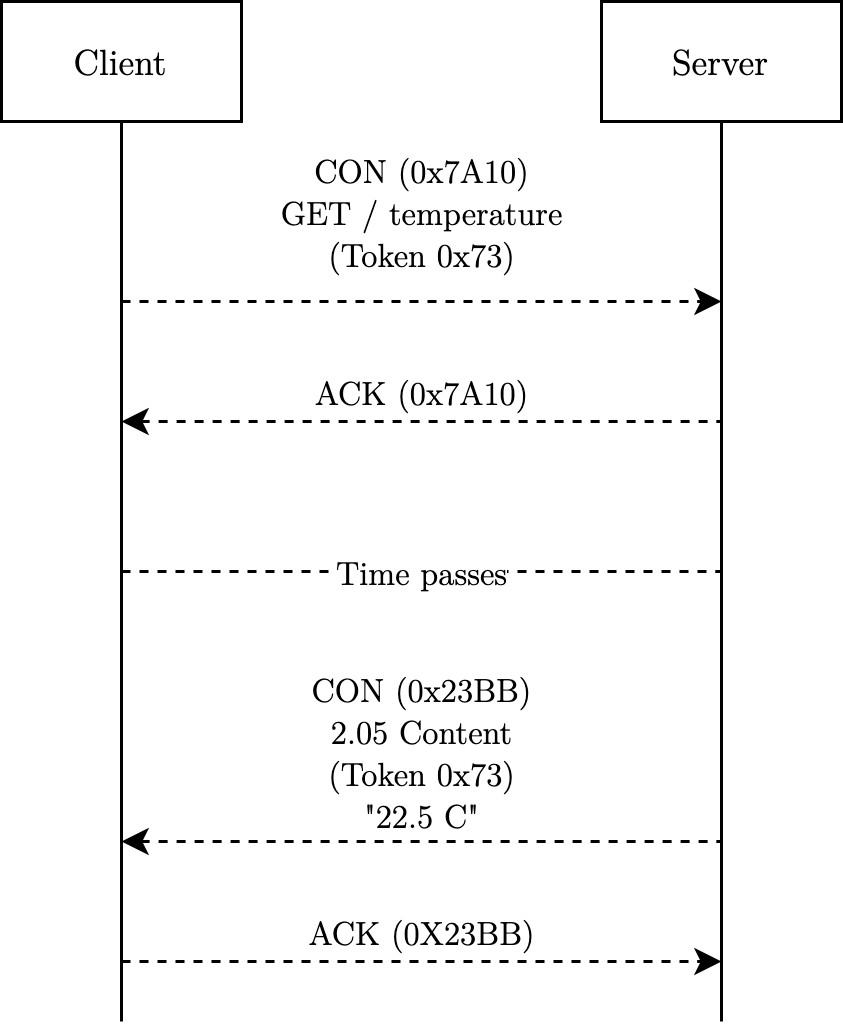
\includegraphics [scale=0.175] {separatereqres.png}
	\caption{A GET Request with a Separate Response}
\end{figure}
\end{itemize}
In case the message used in the request was a Non-confirmable (NON), the response is also a Non-confirmable (NON) message, although the server may instead send a Confirmable (CON) message.
\begin{figure}[H]
	\centering
	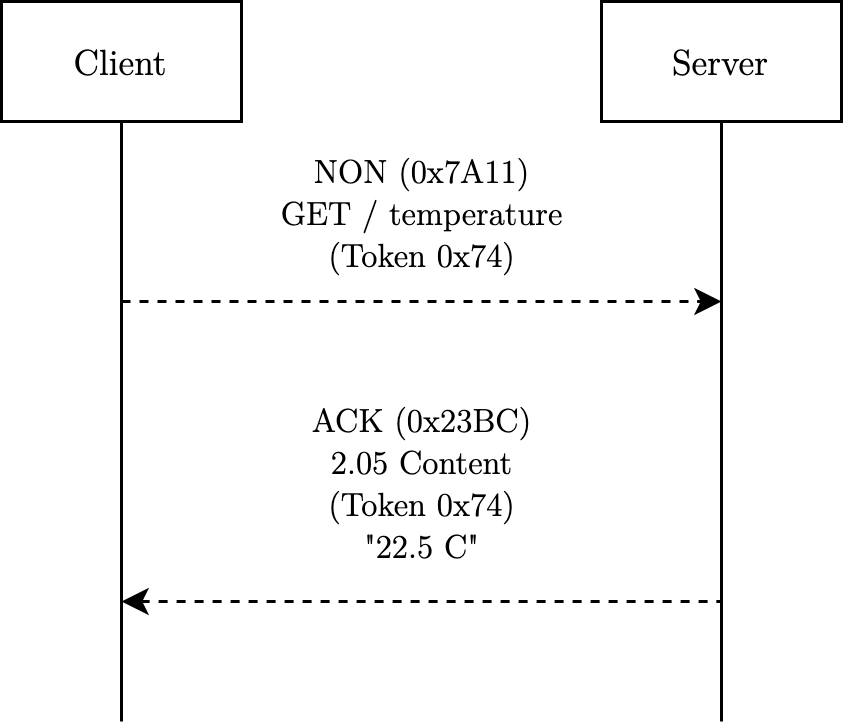
\includegraphics [scale=0.175] {nonreqres.png}
	\caption{A Request and a Response Carried in Non-confirmable Messages}
\end{figure}

\subsubsection{URI scheme}
CoAP uses the "coap" and "coaps" URI schemes for identifying CoAP resources and providing a means of locating the resource. 
\begin{center}
\texttt{coap-URI = "coap:" "//" host [ ":" port ] path-abempty [ "?" query ]}\\
\texttt{coaps-URI = "coaps:" "//" host [ ":" port ] path-abempty
               [ "?" query ]}
\end{center}
\begin{itemize}
\item \textbf{host:} it can be an IP address or a registered depending on the host and it is necessary to identify said host. 
\item \textbf{port:} indicates the UDP port at which the CoAP server is located.  If it is empty or not given, then the default port 5683 is assumed.
\item \textbf{path:} identifies a resource within the scope of the host and port. It consists of a sequence of path segments separated by a slash character (U+002F SOLIDUS "/").
\item \textbf{query:} serves to further parameterise the resource.  It consists of a sequence of arguments separated by an ampersand character (U+0026 AMPERSAND "\&").  An argument is often in the form of a ``key=value" pair.
\end{itemize}

\subsubsection{Response codes}
\begin{center}
\begin{tabular}{ |p{3cm}|p{6cm}|  }
 \hline
 \textbf{Code} & \textbf{Description} \\
 \hline
 65 & 2.01 Created \\
 66 & 2.02  Deleted\\
 67 & 2.03 Valid\\
 68 & 2.04 Changed\\
 69 & 2.05  Content\\
 128 & 4.00  Bad Request\\
 129 & 4.01 Unauthorised\\
 130 & 4.02 Bad Option\\
 131 & 4.03 Forbidden\\
 132 & 4.04 Not Found\\
 133 & 4.05 Method Not Allowed\\
 134 & 4.06 Not Acceptable\\
 140 & 4.12 Precondition Failed\\
 141 & 4.13 Request Entity Too Large\\
 143 & 4.15 Unsupported Content-Format\\
 160 & 5.00 Internal Server Error\\
 161 & 5.01 Not Implemented\\
 162 & 5.02 Bad Gateway\\
 163 & 5.03 Service Unavailable\\
 164 & 5.04 Gateway Timeout\\
 165 & Proxying Not Supported\\
\hline
\end{tabular}
\caption{Table to test captions and labels}
\label{table:1}
\end{center}
\section{Securing CoAP}
\subsection{DTLS: Datagram Transport Layer Security}
\chapter{Test - Setup}
\chapter{Test - Analysis}
\chapter{Conclusion}
\chapter{Discussion}

\end{document}
